\documentclass[12pt]{article}
\usepackage{amsmath}
\usepackage{amssymb}
\usepackage[letterpaper,margin=0.85in,centering]{geometry}
\usepackage{fancyhdr}
\usepackage{enumerate}
\usepackage{lastpage}
\usepackage{multicol}
\usepackage{graphicx}

\reversemarginpar

\pagestyle{fancy}
\cfoot{Page \thepage \ of \pageref{LastPage}}\rfoot{{\bf Total Points: 60}}
\chead{MATH 1410A}\lhead{Test \# 1}\rhead{Tuesday, 7\textsuperscript{th} February, 2017}

\newcommand{\points}[1]{\marginpar{\hspace{24pt}[#1]}}
\newcommand{\skipline}{\vspace{12pt}}
%\renewcommand{\headrulewidth}{0in}
\headheight 30pt

\newcommand{\di}{\displaystyle}
\newcommand{\R}{\mathbb{R}}
\newcommand{\aaa}{\mathbf{a}}
\newcommand{\bbb}{\mathbf{b}}
\newcommand{\ccc}{\mathbf{c}}
\newcommand{\dotp}{\boldsymbol{\cdot}}
\newcommand{\abs}[1]{\lvert #1\rvert}
\newcommand{\len}[1]{\lVert #1\rVert}
\newcommand{\ivec}{\,\boldsymbol{\hat{\imath}}}
\newcommand{\jvec}{\,\boldsymbol{\hat{\jmath}}}
\newcommand{\kvec}{\,\boldsymbol{\hat{k}}}
\newcommand{\bvm}{\begin{vmatrix}}
\newcommand{\evm}{\end{vmatrix}}

\DeclareMathOperator{\comp}{comp}

\begin{document}

\author{Instructor: Sean Fitzpatrick}
\thispagestyle{plain}
\begin{center}
\emph{University of Lethbridge}\\
Department of Mathematics and Computer Science\\
7\textsuperscript{th} February, 2017, 1:45 - 2:55 pm\\
{\bf MATH 1410A - Test \#1}\\
\end{center}
\skipline \skipline \skipline \noindent \skipline
Last Name:\underline{\hspace{353pt}}\\
\skipline
First Name:\underline{\hspace{350pt}}\\
\skipline
Student Number:\underline{\hspace{323pt}}\\
\skipline
Tutorial Time: \underline{\hspace{320pt}}\\


\vspace{0.5in}


\begin{quote}
  Record your answers below each question in the space provided.    Left-hand pages may be used as scrap paper for rough work.  If you want any work on the left-hand pages to be graded, please indicate so on the right-hand page.
 
 \bigskip
 
To earn partial credit, you must show your work. Correct answers without adequate justification in most cases do not receive full marks.

\bigskip

{\bf No external aids are allowed, with the exception of a 5-function calculator.}
\end{quote}


\vspace{0.5in}

For grader's use only:

\begin{table}[hbt]
\begin{center}
\begin{tabular}{|l|r|} \hline
Page&Grade\\
\hline \hline
\cline{1-2} 2 & \enspace\enspace\enspace\enspace\enspace\enspace/12\\
\cline{1-2} 3 & \enspace\enspace\enspace\enspace\enspace\enspace/12\\
\cline{1-2} 4 & \enspace\enspace\enspace\enspace\enspace\enspace/12\\
\cline{1-2} 5 & \enspace\enspace\enspace\enspace\enspace\enspace/12\\
\cline{1-2} 6 & \enspace\enspace\enspace\enspace\enspace\enspace/12\\
\cline{1-2} Total & \enspace\enspace\enspace\enspace\enspace\enspace/60\\
\hline
\end{tabular}

\skipline

\skipline

\skipline


\end{center}
\end{table}
\newpage


\begin{enumerate}
 \item True/False problems: for each statement below, indicate if it is true or false. If it is true, explain why. If it is false, give an example where the statement fails to hold. (Remember that ``true'' means true \textbf{in general}. A statement is false if it fails in even one case.) 

 \begin{enumerate}
  \item For any complex numbers $z$ and $w$, $\abs{z+w} = \abs{z}+\abs{w}$. \points{3}

\vspace{1.75in}

 \item For any complex numbers $z$ and $w$, $\overline{z+w} = \overline{z} + \overline{w}$. \points{3}

\vspace{1.75in}

 \item If $\vec{a}\dotp\vec{b}=0$ for two vectors $\vec{a},\vec{b}$ in $\R^2$, then either $\vec{a}=\vec{0}$, or $\vec{b}=\vec{0}$.\points{3}

\vspace{1.75in}

 \end{enumerate}

 \item Define what it means for a vector $\vec{v}$ in $\R^3$ to be a \textbf{unit vector}.\points{3}

\newpage

\item Given the complex numbers $z=4+5i$ and $w=-2+3i$, compute the following. You do not need to explain your work.
 \begin{enumerate}
\item $z+w$ \points{2}

\vspace{1in}

\item $\overline{z}$ \points{2}

\vspace{1in}

\item $\abs{w}$ \points{2}

\vspace{1.25in}

\item $zw$ \points{3}

\vspace{1.25in}

\item $\dfrac{z}{w}$ \points{3}


\end{enumerate}

\newpage

\item Given the vectors $\vec{v} = \langle 4,3,-5\rangle$ and $\vec{w} = \langle -2,1,0\rangle$, compute the following. You do not need to explain your work.
\begin{enumerate}
 \item $2\vec{v}-5\vec{w}$  \points{2}

\vspace{1in}
  
 \item $\len{\vec{v}}$ \points{2}

\vspace{1in}

 \item $\vec{v}\dotp\vec{w}$ \points{2}

\vspace{1in}

 \item $\vec{v}\times \vec{w}$ \points{3}

\vspace{2.5in}

 \item $\operatorname{proj}_{\vec{v}}\vec{w}$ \points{3}
\end{enumerate}
\newpage



 \item \begin{enumerate}
\item Convert the complex number $z=-1+\sqrt{3}\,i$ to polar form. \points{3}

\vspace{2in}

\item Convert the complex number $w=4e^{i(\pi/4)}$ to rectangular form. \points{2}

\vspace{1.5in}

 \item Compute the value of $z^8$, where $z$ is as given in part (a).\points{4}\\
 Express your answer in rectangular form. 

\vspace{2.25in}

 \item Compute the value of $\dfrac{z^2}{w^3}$, where $z$ and $w$ are as given in parts (a) and (b). \points{3}\\
Express your answer in polar form. 
\end{enumerate}
\newpage

\item \begin{enumerate}
\item Find the vector equation of the line $\ell$ that passes through the points $P=(3,2,-4)$ and $Q=(5,1,2)$. \points{3}

\vspace{2.25in}

\item Find the scalar equation of the plane $\mathcal{P}$ that passes through the points $A=(1,-2,4)$, $B=(3,0,5)$, and $C = (1,-1,2)$. \points{5}

\vspace{3.5in}

\item Find the point of intersection between the line $\ell$ and the plane $\mathcal{P}$ determined above. \points{4}

\end{enumerate}

\newpage

Extra space for rough work. You may remove this page.

\vspace{4in}

\begin{center}
 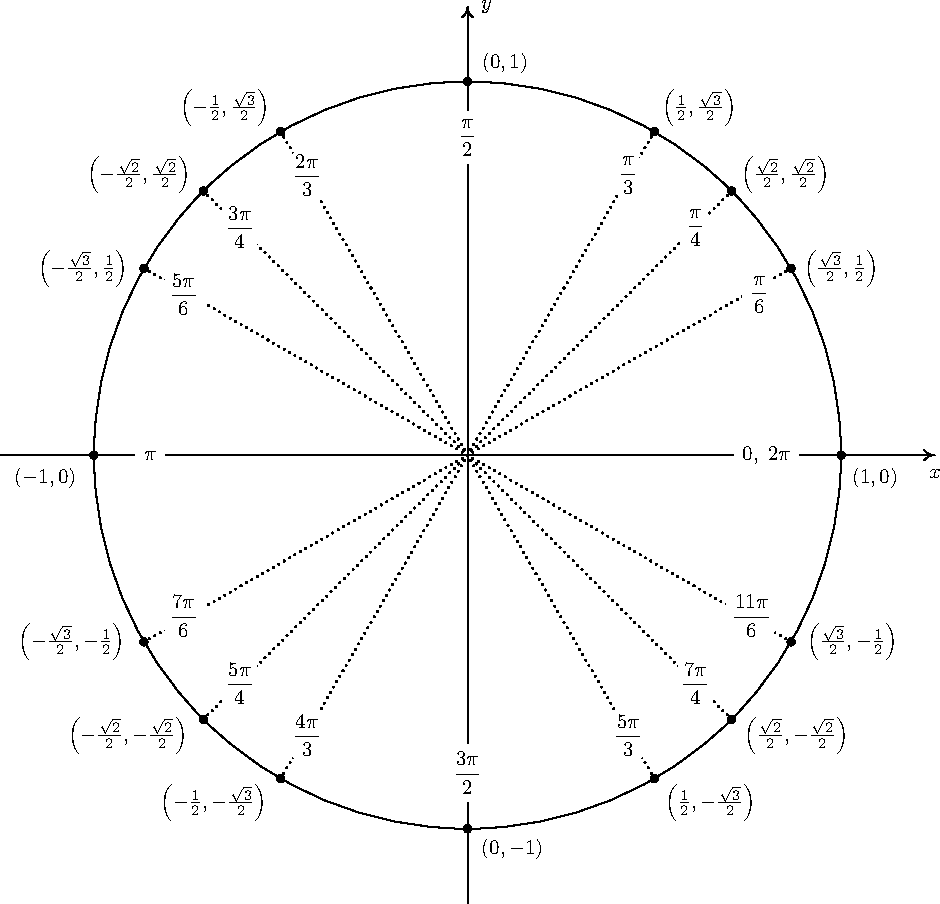
\includegraphics[width=5in]{UnitCircle}
\end{center}


\end{enumerate}
\end{document}